
\subsection{Shortest Job First}
\markright{\thesubsection\quad Shortest Job First} % Manually update \rightmark


\subsubsection{Turnaround time}

From \cref{fig:sjfTurnDensity} we observe that all distributions, even when $\rho = 0.9$ resemble an exponential distribution, in contrast to the \texttt{FCFS} case.

\begin{figure}[H]
    \captionsetup{type=figure}
    \centering
    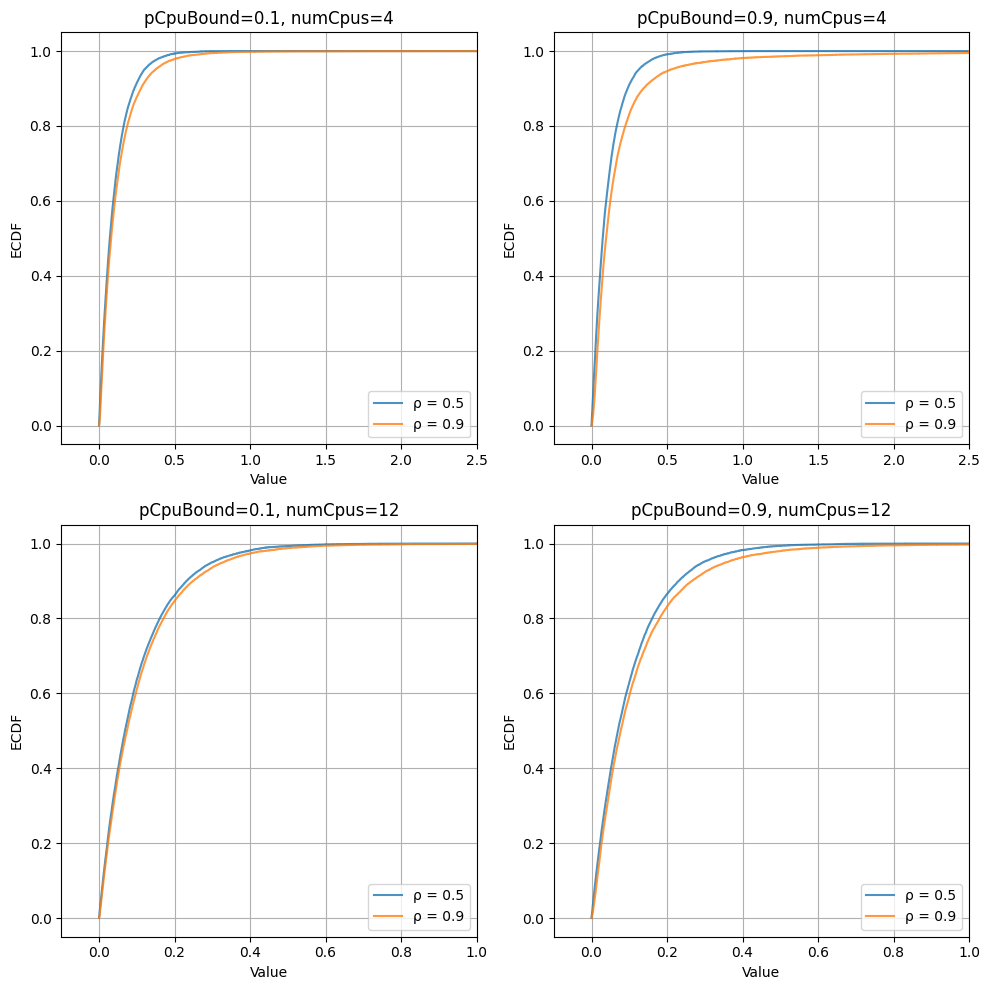
\includegraphics[width=0.9\textwidth]{./images/04/sjf/turn/ecdf.png}
    \caption{Empirical CDF of the turnaround time of the systems.}
    \label{fig:sjfTurnEcdf}
\end{figure}

\begin{figure}[H]
    \captionsetup{type=figure}
    \centering
    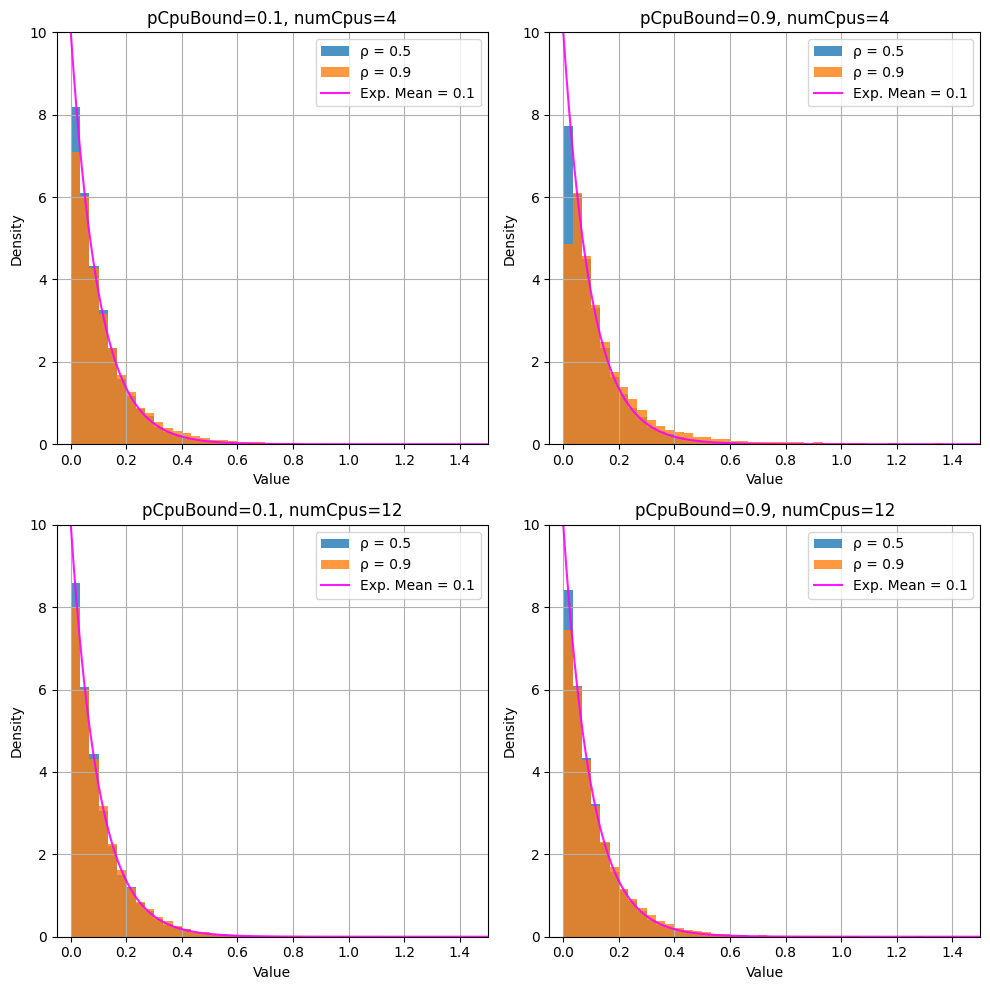
\includegraphics[width=0.9\textwidth]{./images/04/sjf/turn/density.png}
    \caption{Density plot of the turnaround time of the systems.}
    \label{fig:sjfTurnDensity}
\end{figure}

\begin{figure}[H]
    \captionsetup{type=figure}
    \centering
    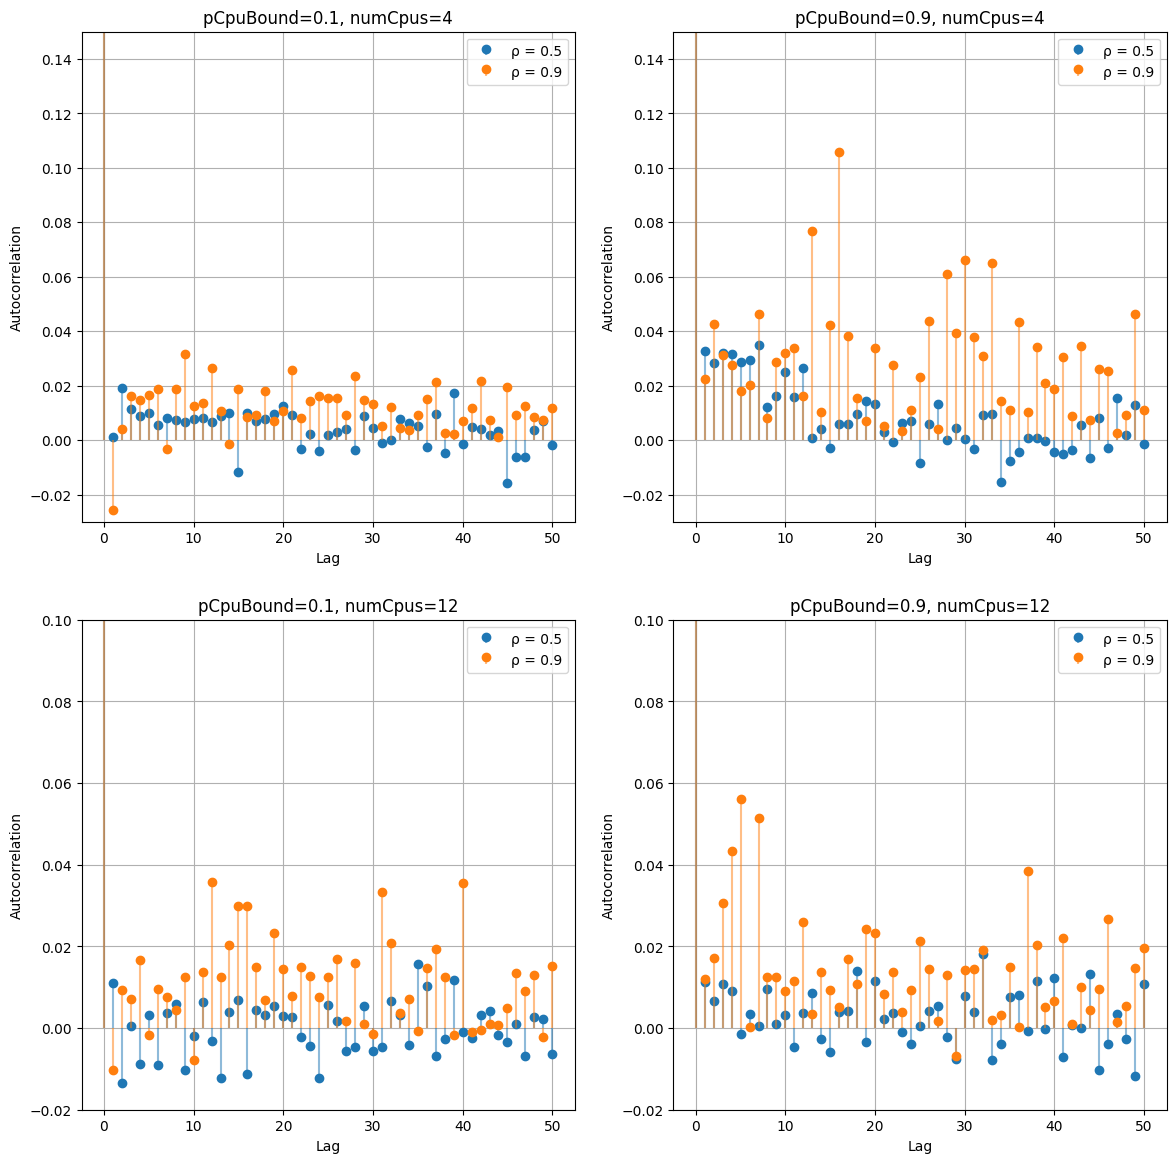
\includegraphics[width=0.9\textwidth]{./images/04/sjf/turn/autocorrelation.png}
    \caption{Autocorrelation plot of the turnaround time of the systems.}
    \label{fig:sjfTurnAutocorrelation}
\end{figure}

\begin{figure}[H]
    \captionsetup{type=figure}
    \centering
    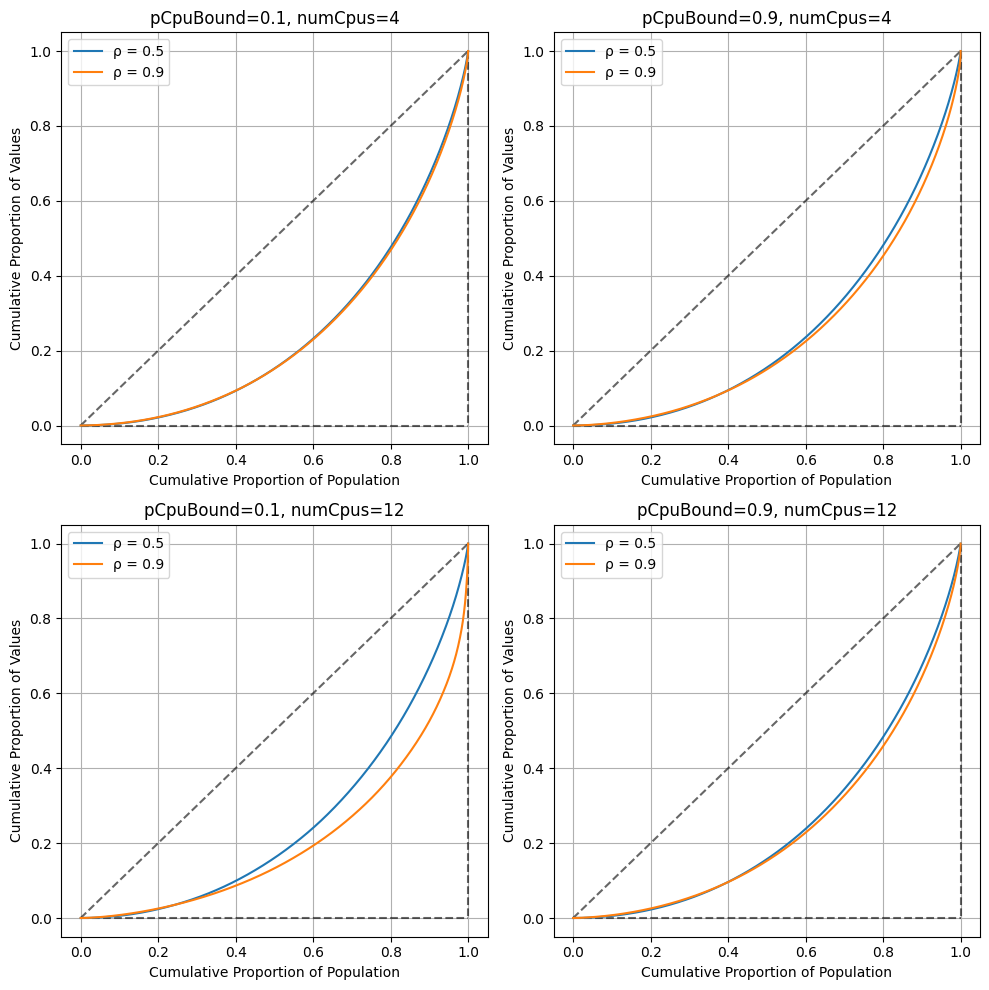
\includegraphics[width=0.9\textwidth]{./images/04/sjf/turn/lorenz.png}
    \caption{Lorenz curve of the turnaround time of the systems.}
    \label{fig:sjfTurnLorenz}
\end{figure}


\begin{table}[H]
    \centering
    \scriptsize
    \begin{tabular}{llc|c|c|c|c|c|c|c}
\toprule
& & \multicolumn{4}{c|}{numCpus = 4} & \multicolumn{4}{c}{numCpus = 12} \\
& & \multicolumn{2}{c|}{pCpuBound = 0.1} & \multicolumn{2}{c|}{pCpuBound = 0.9} & \multicolumn{2}{c|}{pCpuBound = 0.1} & \multicolumn{2}{c}{pCpuBound = 0.9} \\
Index & & $\rho = 0.5$ & $\rho = 0.9$ & $\rho = 0.5$ & $\rho = 0.9$ & $\rho = 0.5$ & $\rho = 0.9$ & $\rho = 0.5$ & $\rho = 0.9$ \\
\midrule
\multirow{3}{*}{Mean} & Value & 102.2 & 123.3 & 105.7 & 168.4 & 98.7 & 107.7 & 100.0 & 120.1 \\
 & 95\% CI Low & 100.4 & 117.7 & 102.0 & 157.6 & 97.0 & 103.3 & 98.5 & 114.3 \\
 & 95\% CI High & 104.3 & 129.6 & 110.0 & 180.7 & 100.7 & 112.8 & 101.2 & 127.6 \\
\midrule
\multirow{3}{*}{Std Dev} & Value & 100.0 & 142.3 & 106.9 & 294.2 & 97.2 & 123.4 & 98.9 & 169.4 \\
 & 95\% CI Low & 97.7 & 129.9 & 101.0 & 253.6 & 94.8 & 113.3 & 97.2 & 128.5 \\
 & 95\% CI High & 102.8 & 170.4 & 113.8 & 354.2 & 99.8 & 146.7 & 100.8 & 258.6 \\
\bottomrule
\end{tabular}
    \caption{Bootstrap results for turnaround time mean and Std Dev. (ms)}
    \label{tab:sjfTurn}
\end{table}


\subsubsection{Waiting time}


\begin{figure}[H]
    \captionsetup{type=figure}
    \centering
    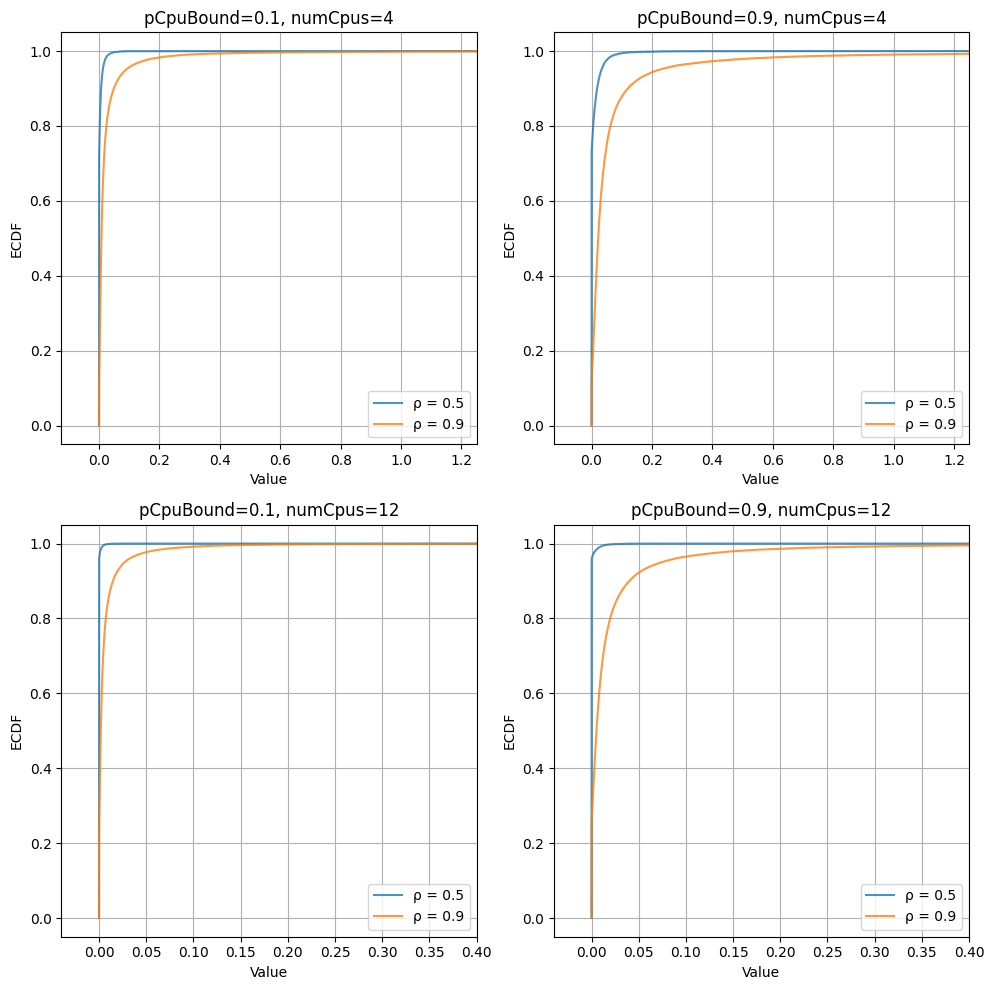
\includegraphics[width=0.9\textwidth]{./images/04/sjf/wait/ecdf.png}
    \caption{Empirical CDF of the waiting time of the systems.}
    \label{fig:sjfWaitEcdf}
\end{figure}

\begin{figure}[H]
    \captionsetup{type=figure}
    \centering
    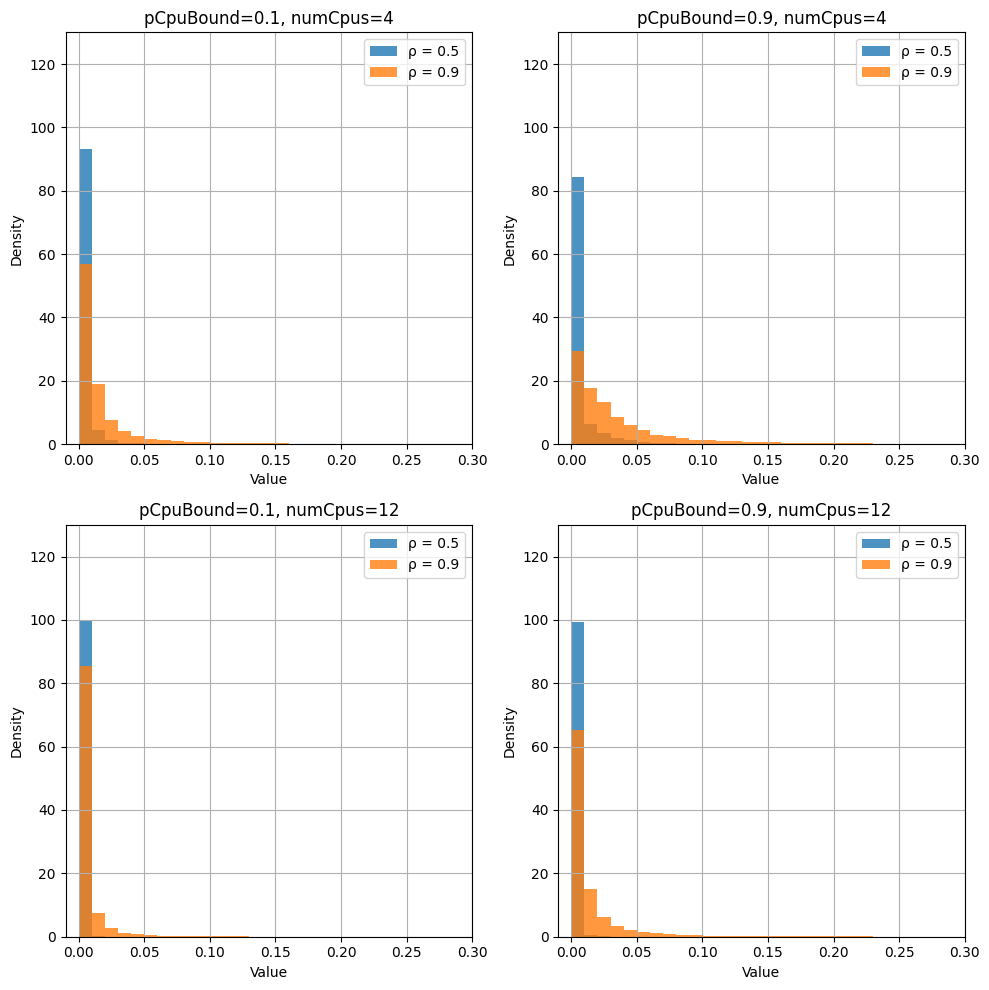
\includegraphics[width=0.9\textwidth]{./images/04/sjf/wait/density.png}
    \caption{Density plot of the waiting time of the systems.}
    \label{fig:sjfWaitDensity}
\end{figure}

\begin{figure}[H]
    \captionsetup{type=figure}
    \centering
    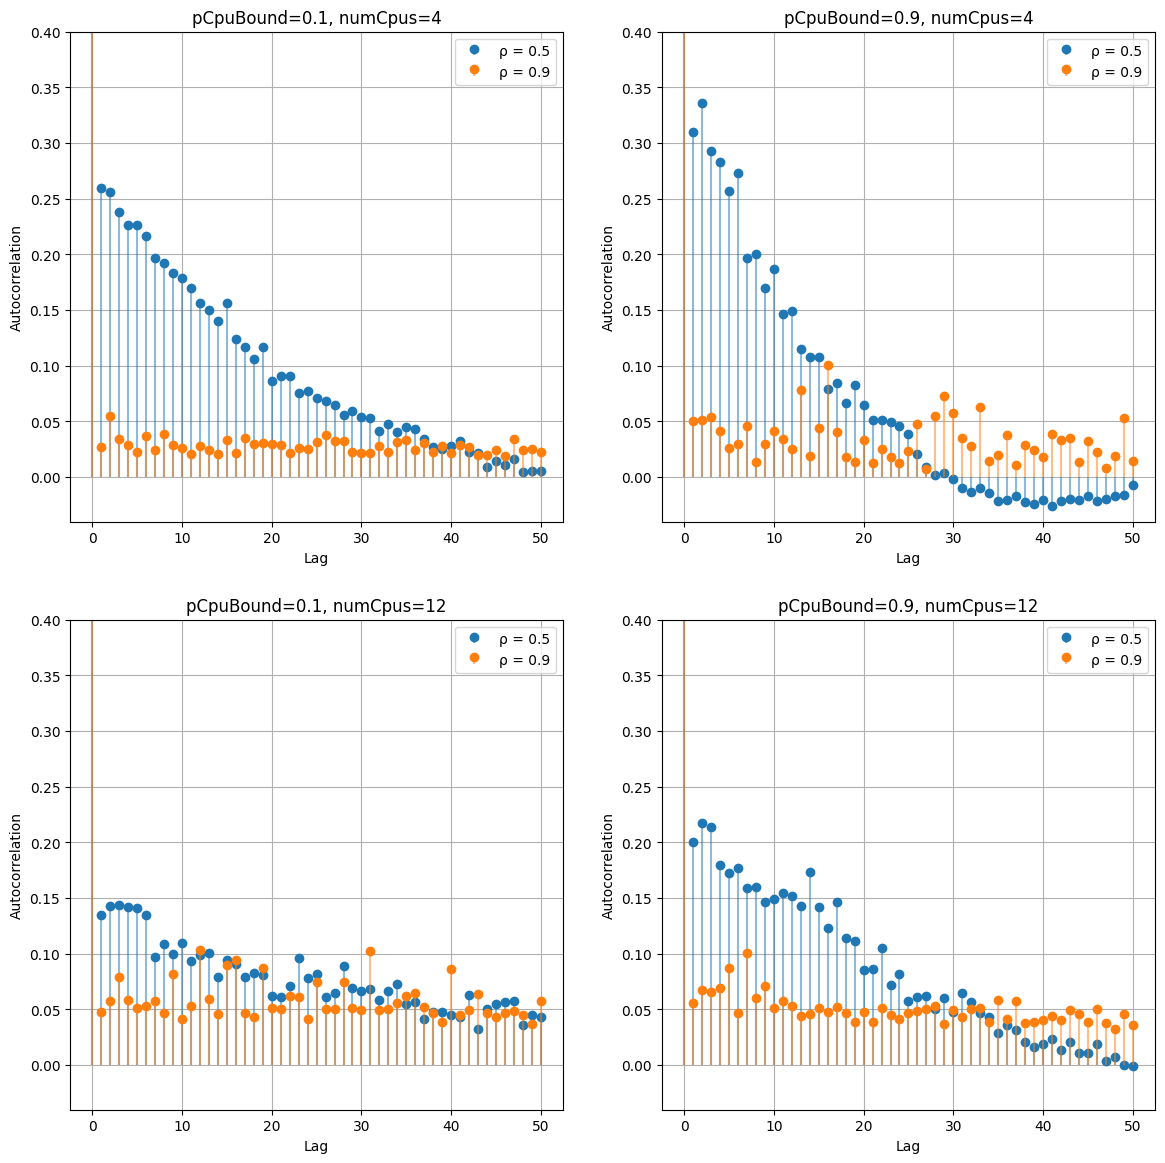
\includegraphics[width=0.9\textwidth]{./images/04/sjf/wait/autocorrelation.png}
    \caption{Autocorrelation plot of the waiting time of the systems.}
    \label{fig:sjfWaitAutocorrelation}
\end{figure}

\begin{figure}[H]
    \captionsetup{type=figure}
    \centering
    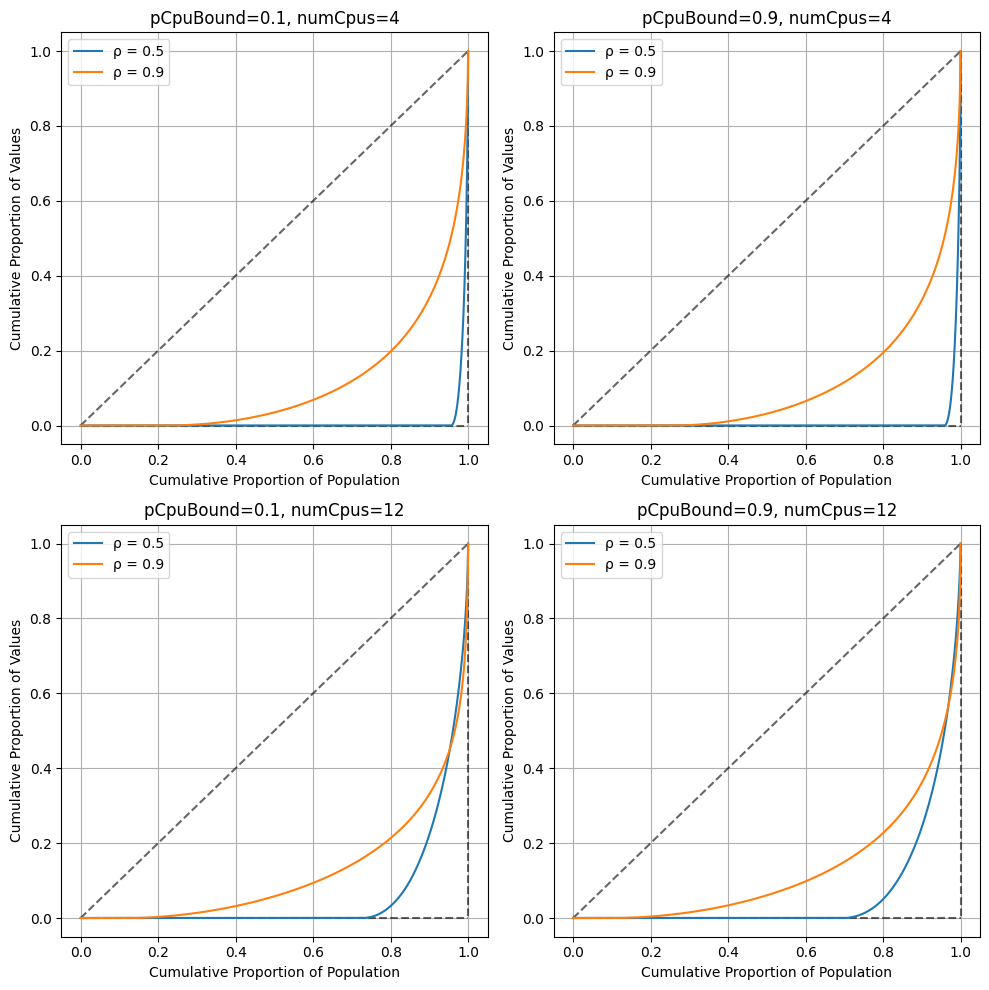
\includegraphics[width=0.9\textwidth]{./images/04/sjf/wait/lorenz.png}
    \caption{Lorenz curve of the waiting time of the systems.}
    \label{fig:sjfWaitLorenz}
\end{figure}


\begin{table}[H]
    \centering
    \scriptsize
    \begin{tabular}{llc|c|c|c|c|c|c|c}
\toprule
& & \multicolumn{4}{c|}{numCpus = 4} & \multicolumn{4}{c}{numCpus = 12} \\
& & \multicolumn{2}{c|}{pCpuBound = 0.1} & \multicolumn{2}{c|}{pCpuBound = 0.9} & \multicolumn{2}{c|}{pCpuBound = 0.1} & \multicolumn{2}{c}{pCpuBound = 0.9} \\
Index & & $\rho = 0.5$ & $\rho = 0.9$ & $\rho = 0.5$ & $\rho = 0.9$ & $\rho = 0.5$ & $\rho = 0.9$ & $\rho = 0.5$ & $\rho = 0.9$ \\
\midrule
\multirow{3}{*}{Mean} & Value & 2.2 & 26.4 & 4.5 & 78.5 & 0.1 & 6.2 & 0.2 & 18.9 \\
 & 95\% CI Low & 1.9 & 23.6 & 3.6 & 67.4 & 0.1 & 5.4 & 0.1 & 16.9 \\
 & 95\% CI High & 2.8 & 32.1 & 5.7 & 105.5 & 0.1 & 7.4 & 0.3 & 23.9 \\
 \midrule
 \multirow{3}{*}{Std Dev} & Value & 6.7 & 112.6 & 13.2 & 430.3 & 0.5 & 19.3 & 1.7 & 86.7 \\
 & 95\% CI Low & 5.1 & 72.4 & 10.9 & 260.8 & 0.4 & 14.2 & 1.1 & 46.5 \\
 & 95\% CI High & 10.3 & 192.6 & 18.8 & 801.1 & 0.6 & 28.0 & 3.2 & 177.7 \\
\bottomrule
\end{tabular}
    \caption{Bootstrap results for waiting time mean and Std Dev. (ms)}
    \label{tab:sjfWait}
\end{table}


\subsubsection{CPU utilization}

There is no difference with \cref{sec:fcfsCpuUtilization} since the \texttt{FCFS}and \texttt{SJF} schedulers have the same behaviour in terms of CPU utilization.

\subsubsection{Ready queue length}

\begin{table}[H]
    \centering
    \scriptsize
    \begin{tabular}{lc|c|c|c|c|c|c|c}
\toprule
& \multicolumn{4}{c|}{numCpus = 4} & \multicolumn{4}{c}{numCpus = 12} \\
& \multicolumn{2}{c|}{pCpuBound = 0.1} & \multicolumn{2}{c|}{pCpuBound = 0.9} & \multicolumn{2}{c|}{pCpuBound = 0.1} & \multicolumn{2}{c}{pCpuBound = 0.9} \\
Index & $\rho = 0.5$ & $\rho = 0.9$ & $\rho = 0.5$ & $\rho = 0.9$ & $\rho = 0.5$ & $\rho = 0.9$ & $\rho = 0.5$ & $\rho = 0.9$ \\
\midrule
Mean & 0.17 & 3.54 & 0.16 & 3.47 & 0.02 & 3.12 & 0.02 & 2.93 \\
\midrule
Std Dev & 0.66 & 3.62 & 0.62 & 3.57 & 0.23 & 4.03 & 0.23 & 3.80 \\
\bottomrule
\end{tabular}
    \caption{Mean and Std Dev of number of ready processes in queue.}
    \label{tab:sjfReadyProc}
\end{table}
